
\documentclass{article}
\usepackage{graphicx}
\usepackage{amsmath}

\usepackage{amssymb}
\usepackage{natbib}
\usepackage{subfigure}
\usepackage{epsfig}
\bibliographystyle{harvard}


\title{A Decomposition of the Bradley-Blackwood Paired-Samples Test}

\author{Kevin Hayes%\footnote{Kevin Hayes is Lecturer in Statistics, Department %of Mathematics and Statistics, University of Limerick, Limerick. Ireland. %(E-mail: \textit{kevin.hayes@ul.ie}).}
\and Kevin O'Brien  \and Anthony Kinsella}
\date{ }

\renewcommand{\baselinestretch}{1}
\textwidth 27pc


\begin{document}

\maketitle

%\newpage

\begin{abstract}
In this article, we show that the Bradley-Blackwood simultaneous test for equal means and equal variances in paired-samples decomposes additively into separate tests on the composite hypotheses. The test of equal variances arising in this decomposition is the standard Pitman-Morgan procedure. The test of equal means is based on a \textit{t}-ratio with $(n-2)$ degrees of freedom, and is shown to have an advantage in terms of power over the classic paired-samples Student  \textit{t}-test in cases of unequal variances. Some implications for simultaneous inference are discussed. \\ KEY WORDS: Centered regression; Pitman-Morgan; Simultaneous inference.
\end{abstract}

\bigskip

\section{INTRODUCTION}

Let the random variables $Y_1$ and $Y_2$ be distributed bivariate normal with $\mathrm{E}(Y_1)=\mu_1,$ $\mathrm{E}(Y_2)=\mu_2,$ $\mathrm{var}(Y_1)=\sigma_1,$ $\mathrm{var}(Y_2)=\sigma_2,$ and correlation coefficient $-1<\rho_{12}<1.$ Of interest are tests of the marginal hypotheses H$'$: $\mu_1-\mu_2=0$ and H$''$: $\sigma^2_1 =\sigma^2_2,$ and tests of the joint hypothesis H$^{\textrm{J}}$: $\mu_1-\mu_2=0$ and $\sigma^2_1=\sigma^2_2.$ The random variables $D=Y_1-Y_2$ and $S=Y_1+Y_2$ are bivariate normal with expectations $\mathrm{E}(D)=\mu_D= \mu_1-\mu_2$ and $\mathrm{E}(S)=\mu_S= \mu_1+\mu_2,$ variances $\mathrm{var}(D) =\sigma^2_D= \sigma_1^2+ \sigma_2^2 -2\rho_{12}\sigma_1 \sigma_2$ and $ \mathrm{var}(S) = \sigma^2_S =\sigma_1^2+ \sigma_2^2 +2\rho_{12}\sigma_1 \sigma_2,$ and covariance $\mathrm{cov}(D,S) = \sigma_1^2 - \sigma_2^2.$ These random variables differences and sums are the building blocks of the test procedures: for H$'$, due to \cite{Student}; for H$''$, devised concurrently by \cite{Pit39} and \cite{Morgan39}; and for H$^{\textrm{J}}$ due to \cite{BradBlack89}.

In this article we show that the test of the hypothesis H$^{\textrm{J}}$ due to \cite{BradBlack89} decomposes additively into independent tests of H$'$ and H$''$. The latter test is identical to the Pitman-Morgan procedure above. The former test is based on a t-ratio with $(n-2)$df, denoted below by $t_0^\ast,$ and has an advantage in terms of power over the classical paired-samples Student \textit{t}-test in cases where $\sigma_1^2 \neq \sigma_2^2.$

The remainder of the paper is structured as follows. In the next section we
use the notation of the random variables $D$ and $S$ to motivate the tests of the aforementioned hypotheses. The decomposition of the Bradley-Blackwood test is given in section 3. In section 4 we compare the power functions of the paired-samples Student \textit{t}-test and the test based on the \emph{t}-tatio $t_0^\ast$. Some implications for simultaneous inference about $\mu_1-\mu_2$ and $\sigma^2_1 - \sigma^2_2$ are discussed in section 5. We conclude the paper with some simple examples.

\bigskip

\section{TESTS}

\subsection{Student's \textit{t}-Test}

The test of the hypothesis H$'$: $\mu_D=0$ due to \cite{Student} is based on the \emph{t}-ratio
\begin{equation}
\label{StudentT} t^\ast = \frac{ \bar{d} }{ \hat{\sigma}/ \sqrt{n}} \sim t_{(n-1)\textrm{df}},
\end{equation}
where $\bar{d}$ is the mean of the $n$ case-wise differences $d_i=y_{i1}-y_{i2}$ of the observed pairs $(y_{i1},y_{i2}),\ i=1,\ldots,n$ and
\[
\hat{\sigma}^2 = \frac{1}{ n-1} \sum_{i=1}^n (d_i-\bar{d})^2
\]
is the usual estimate of the variance of the differences $\sigma^2_D.$ This classical test makes no assumptions about the equality (or otherwise) of the variance parameters $\sigma^2_1$ and $\sigma^2_2.$


\subsection{The Pitman-Morgan Test}

The test of the hypothesis that the variances $\sigma^2_1$ and $\sigma^2_2$ are equal, which was devised concurrently by \cite{Pit39} and \cite{Morgan39}, is based on the correlation of $D$ with $S,$ the coefficient being $ \rho_{DS} = (\sigma^2_1 -\sigma^2_2) / ( \sigma_D \sigma_S ),$ which is zero if, and only
if, $\sigma^2_1 = \sigma^2_2.$ Consequently a test of H$''$: $\sigma^2_1 = \sigma^2_2$ is equivalent to a test of H$''$: $\rho_{DS}=0$ and the test statistic is the familiar {\it t}-test for a correlation coefficient with $(n-2)$ degrees of freedom.

\subsection{The Bradley-Blackwood Test}

\cite{BradBlack89} write the conditional expectation of $D$ given $S$ as
\begin{eqnarray*}
\mathrm{E}(D|S) & = & \mu_D + \mathrm{cov}(D,S)
    \mathrm{var}(S)^{-1}(S-\mu_S), \nonumber \\
    & = & \mu_D + [(\sigma^2_1-\sigma^2_2)/ \sigma^2_S]
    (S - \mu_S),\\
    & = &\beta_0 + \beta_1 S,
\end{eqnarray*}
where $\beta_0=\mu_D-[(\sigma^2_1-\sigma^2_2)/ \sigma^2_S] \mu_S$ and $\beta_1 = (\sigma^2_1-\sigma^2_2)/ \sigma^2_S.$ Bradley and Blackwood used this result to propose a test of the joint hypothesis H$^{\textrm{J}}$: $\mu_D = 0$ and $\sigma^2_1 = \sigma^2_2,$ which is true if, and only if, $\beta_0=\beta_1=0.$ The test statistic is
\begin{equation}\label{BB:Fstat}
F^* = [(\sum{d_i^2} - \mathrm{SSE})/2]/[\mathrm{SSE}/(n-2)] \sim
F_{(2,n-2)\textrm{df}},
\end{equation}
where $\sum{d_i^2}$ is the sum of the squares of the $n$ observed differences, and $\mathrm{SSE}$ is the residual error sum-of-squares from the regression $\hat{d}_i=\hat{\beta}_0 +\hat{\beta}_1 s_i$ of the observed case-wise differences on the case-wise sums. They also note that the Pitman-Morgan test of the marginal hypothesis H$''$: $\sigma^2_1 = \sigma^2_2,$  is identical to
the test of the hypothesis H$''$: $\beta_1=0$ of the slope parameter based on the regression \emph{t}-ratio
\begin{equation}
\label{tOne} t_1^\ast = \frac{ \hat\beta_1 }{ \tilde{\sigma} /
\sqrt{\sum{(s_i-\bar{s})^2}}} \sim t_{(n-2)\textrm{df}},
\end{equation}
where $\tilde{\sigma}^2 = \mathrm{SSE}/(n-2)$ is the mean square error from the regression of differences on sums.

\bigskip

\section{DECOMPOSITION OF THE BRADLEY-BLACKWOOD TEST}

The residual sum-of-squares can be written
\[
\mathrm{SSE} = \sum_{i=1}^n(d_i-\bar{d})^2 - \hat{\beta}^2
\sum_{i=1}^n (s_i-\bar{s})^2 ,
\]
and using the identity $\sum (d_i-\bar{d})^2=\sum d_i^2 - n\bar{d}^2$   the numerator in (\ref{BB:Fstat}) can be further rewritten $[ n\bar{d}^2 + \hat{\beta}^2 \sum (s_i-\bar{s})^2]/2.$ The Bradley-Blackwood test statistic
from (\ref{BB:Fstat}) can now be expressed in the more intuitive form
\begin{equation} \label{BBHayes}
F^\ast = [\ (t_0^\ast)^2 + (t_1^\ast)^2\ ] /2 \sim
F_{(2,n-2)\textrm{df}},
\end{equation}
where $t_1^\ast$ is the Pitman-Morgan test statistic from (\ref{tOne}), and the \textit{t}-ratio
\begin{equation}
\label{tZero} t_0^\ast = \frac{ \bar{d} }{ \tilde{\sigma}/\sqrt{n}}
\sim t_{(n-2)\textrm{df}}
\end{equation}
is a test of the marginal hypothesis H$'$: $\mu_D=0,$ and is an alternative to the paired-samples Student \textit{t}-test in (\ref{StudentT}) which is based on $(n-1)$ degrees of freedom.

The t-ratios $t_0^\ast$ and $t_1^\ast$ can be motivated from the `centered' regression $\hat d_i = \hat\gamma_0+\hat\gamma_1 (s_i-\bar{s})$ of the differences against the mean centered case-wise sums $(s_i-\bar{s}).$  Standard results from simple linear regression confirm that for the centered regression model the estimated intercept parameter equals the mean of the case-wise
differences, $\hat\gamma_0 = \bar{d},$ and that the estimated slope parameter is identical to the estimated slope parameter in the non-centered regression $\hat{d}_i=\hat{\beta}_0 +\hat{\beta}_1 s_i$ so that $\hat\gamma_1 = \hat\beta_1.$  The $\mathrm{SSE}$ from the two regressions remains unchanged. It is easy to verify that $\mathrm{Cov}(\bar{d},\hat\beta_1) =
\mathrm{Cov}(\hat\gamma_0,\hat\gamma_1) =0,$ so that independent tests of the hypotheses of equal means and equal variances can be formulated using the regression \textit{t}-ratios.

\bigskip

\section{POWER FUNCTIONS}

The power function for the test of the marginal hypothesis H: $\mu_D=0$ using Student's paired {\it t}-test is characterized by a non-central {\it F}-distribution with degrees of freedom parameters 1 and $(n-1)$ in the numerator and denominator, and non-centrality parameter $ n(\mu_D)^2 / \sigma^2_D.$ The power function for the test of the marginal hypothesis H: $\mu_D=0$ using the regression t-ratio $t_0^\ast$ is a non-central {\it
F}-distribution with degrees of freedom parameters 1 and $(n-2)$ in the numerator and denominator, and non-centrality parameter $ n(\mu_D)^2 / \sigma^2_{D|S},$ where $\sigma^2_{D|S} = \sigma^2_D - (\sigma^2_1-\sigma^2_2 )^2/ \sigma^2_S=\sigma^2_D(1-\rho_{DS}^2)$ is obtained from the conditional distribution of $D|S.$ These results follows as special cases of power functions for tests of the general linear hypothesis in univariate linear models \citep[for example]{Scheffe59}.

For given values of $n$ and $\sigma^2_D$ the non-centrality parameters of these distributions differ by a factor depending only on $\rho^2_{DS},$ which in turn depends on $(\sigma^2_1-\sigma^2_2 )$. In order to compare the power functions of the two tests for different values of $\sigma^2_1$ and $\sigma^2_2,$ it is sufficient to vary the single parameter $\rho_{DS}$ between 0 and 1. These power functions are plotted in Figure \ref{PowerCurves}\subref{PowerOne} and Figure \ref{PowerCurves}\subref{PowerThree} for sample sizes $n = 10$ and
30 respectively, as $\mu_D$ increases from 0 to 1.2, where $\sigma^2_D = 1$ throughout and $\rho_{DS} = 0,\ 0.3,\ 0.6$ and $0.9$. The differences between the power functions of the two tests, obtained by subtracting the power curve for the Student t-test away from the power curve for the regression based test, are plotted in the right-hand-side panels of Figure \ref{PowerCurves}.

When $\rho_{DS}=0,$ that is $\sigma^2_1=\sigma^2_2,$ the Student \textit{t}-test in (\ref{StudentT}) has improved power over the test based on the \textit{t}-ratio in (\ref{tZero}). This can be seen from the negative differences between the power curves shown in Figure \ref{PowerCurves}\subref{PowerTwo} and Figure \ref{PowerCurves}\subref{PowerFour}. For $\rho_{DS}=0$ and $n=10$ the maximum (negative) difference between the power curves equals $0.0135$; for $n=30$ the maximum (negative) difference equals 0.0011. As $\rho_{DS}$ increases, that is $\sigma^2_1 \neq \sigma^2_2,$ the test based on the \textit{t}-ratio (\ref{tZero}) established an advantage in terms of power over the Student
\textit{t}-test in (\ref{StudentT}).

\bigskip

\section{SIMULTANEOUS INFERENCE}

While \cite{BradBlack89} provide a test on the joint hypothesis of equal means and equal variances (model 1, $\mathcal{M}_1$) their regression based approach does not separate these two issues. The rejection of the joint hypothesis may be due to two groups with unequal means and unequal variances ($\mathcal{M}_2$); unequal means and equal variances ($\mathcal{M}_3$), or equal means and unequal variances ($\mathcal{M}_4$).

\subsection{Multiple Testing}

In terms of the \textit{t}-ratios $t_0^\ast$ and $t_1^\ast,$ the region outside the smaller square in Figure \ref{Fig:Rejection:Regions} identifies the simultaneous rejection of the marginal hypotheses H$'$: $\beta_0=0$ and H$''$: $\beta_1 = 0$ when $|t_0^\ast|$ and $|t_1^\ast|$ are simultaneous compared to the cutoff value $t_{\alpha/2,(n-2)\textrm{df}}.$ For illustrative purposes we have chosen $\alpha=0.05$ and $n=20$ so that $t_{\alpha/2,(n-2)\textrm{df}} = 2.101.$ The rejection region for the test of the joint hypothesis H$^{\textrm{J}}$: $\beta_0 =\beta_1=0$ defined by (\ref{BBHayes}) lies outside the circle of radius $r= \sqrt{2F_{\alpha,(2,n-2)\textrm{df}}}$ centered at $(0,0).$ \cite{Krzanowski} uses a similar graphical illustration to demonstrate the pitfalls associated with testing a multivariate hypothesis using a series of univariate tests. The point `P' indicates an occasion when the univariate tests fail to reject the marginal hypotheses but the correct multivariate inference suggests that the joint hypothesis should be rejected. The point `Q' gives rise to the other type of mistake, where the univariate tests lead to the rejection of the (simultaneous) marginal hypotheses, but the correct multivariate inference suggests that the joint hypothesis should not be rejected.

As (\ref{tOne}) and (\ref{tZero}) are independent the collective type I error probability of the univariate tests is not $\alpha=0.05,$ but $1-(1-\alpha)^2 =0.0975$. Although simultaneous testing of these marginal hypotheses could be secured at a collective type I error probability of 0.05 by enlarging the side of the square from $2\times2.101$ to $2\times2.439$, as represented by the outer square in Figure \ref{Fig:Rejection:Regions}, where $2.439=t_{(1- \sqrt{1-\alpha}\ )/2,(n-2)\textrm{df}},$ this would increase the size of the type II error probability. This enlarged test region is identical to a test procedure based on $Z = \max \left\{ (t_0^\ast)^2 , (t_1^\ast)^2 \right\}.$ The quantities $(t_0^\ast)^2$ and $(t_1^\ast)^2$ are independently identically distributed $F_{(1,n-2)\textrm{df}}$.  The random variable $Z$ has probability distribution function $H_Z(z) = G(z)G(z),$ where $G(z)$ is the distribution function of a $F_{(1,n-2)\textrm{df}}$ random variable. The quantile $z$ such that $\mathrm{Pr}(Z<z)=1-\alpha$ can be determined as the $z$ satisfying $G(z) = \sqrt{1-\alpha}.$ The relationship between the $F$ and $t$ distributions identifies the rejection region in this case to coincide with the outer square in Figure \ref{Fig:Rejection:Regions}.

Suppose that the marginal test procedures (\ref{tZero}) and (\ref{tOne}) based on the test statistics $t_0^\ast$ and $t_1^\ast$ lead to \textit{p}-values $P_0$ and $P_1$ respectively. Let $P_{(1)} \leq P_{(2)}$ be the ordered \textit{p}-values and denote by H$_{(i)}$ the null hypothesis corresponding to $P_{(i)}.$ In this setting, the Bonferroni-type multiple testing procedure proposed by \cite{Benjamini95} rejects all H$_{(i)}$, $i=1,\ldots,k$ where $k$ is the largest $i\in \{1,2\}$ for which $P_{(i)} \leq (i/2) q^\star.$ \cite{Benjamini95} show that this test procedure has the desirable property that it controls the false discovery rate, a term attributable to \cite{Soric89}, at a pre-specified level $q^\star.$ For $q^\star = 0.05$, $P_{(1)}$ and $P_{(2)}$ are compared against $\frac{1}{2}0.05$ and $0.05$ respectively. In essence, this approach compares $\max \left\{ |t_0^\ast| , |t_1^\ast| \right\}$ and $\min \left\{ |t_0^\ast| , |t_1^\ast| \right\}$ against the cut-offs $t_{\alpha/4,(n-2)\textrm{df}}$ and $t_{\alpha/2,(n-2)\textrm{df}}$ respectively. The latter cutoff coincides with the rejection region defined by the inner square drawn in Figure \ref{Fig:Rejection:Regions}. The former cutoff defines a square rejection region outside the region defined by the outer square drawn in Figure \ref{Fig:Rejection:Regions}. A choice of model from $\{\mathcal{M}_1, \mathcal{M}_2, \mathcal{M}_3, \mathcal{M}_4\}$ can be made accordingly.


\subsection{Confidence Regions}

Five outcomes of the test statistic pair $(t_0^\ast,t_1^\ast)$  are illustrated in Figure \ref{Fig3a} in the context of the first quadrant. The plotting symbol $\bullet$ lies within the circle determined by (\ref{BB:Fstat}) and $(t_0^\ast,t_1^\ast)$ represent a failure to reject H$^\textrm{J}$. The other four symbols represent situations where H$^\textrm{J}$ is rejected. The position of all five plotting symbols can be interpreted in the context of the following confidence region argument. The elliptical confidence region $n(\beta_0-\hat\beta_0)^2 + [\sum_{i=1}^n(s_i-\bar{s})^2]
(\beta_1-\hat\beta_1)^2 \leq 2\tilde\sigma^2 F_{\alpha,2,n-2}$ for the parameter pair $(\beta_0, \beta_1)$ holds with probability $(1-\alpha),$ see \citet[pg.\ 48]{Myers90}. After some rescaling, the circular confidence region $ (t_0)^2 + (t_1)^2 \leq 2 F_{\alpha,2,n-2}$ centered at $(t_0^\ast,t_1^\ast)$ for the \textit{t}-ratio pair $(t_0, t_1)$ also holds with probability $(1-\alpha)$ and is plotted in Figure \ref{Fig3b}--(f) to illustrate potential inferences that might arise. The $(1-\alpha)100$\% confidence region in Figure \ref{Fig3b} includes the origin supporting $\mathcal{M}_1$, the conclusion that the means are equal and that variances are equal, and is analogous to the plotting symbol $\bullet$ in Figure \ref{Fig3a}. The confidence region in Figure \ref{Fig3c} excludes the origin and does not overlap either axis, supporting $\mathcal{M}_2$, and corresponds to the plotting symbol {\tiny $\blacksquare$} in Figure \ref{Fig3a}. The confidence regions in Figure \ref{Fig3d} and Figure \ref{Fig3e} corresponds to the plotting symbol {$\blacktriangle$} and {$\blacklozenge$} in Figure \ref{Fig3a} and support, respectively, models $\mathcal{M}_1$ and $\mathcal{M}_1$.  The confidence region in Figure \ref{Fig3f} excludes the origin but overlaps both axis, and corresponds to the plotting symbol {$\mathbf{+}$} in Figure \ref{Fig3a}. In this final case model $\mathcal{M}_1$ is discounted, but no explicit choice from  $\{\mathcal{M}_2, \mathcal{M}_3, \mathcal{M}_4\}$ is made.


\subsection*{note...}
In a simulation of 1 million paired-samples for $n=10$ with $\mu_\textrm{D}=0$, $\rho=0.85$, and $\sigma^2_\textrm{D}=1$ the percentages of results in the categories ``b"  through ``f", represented by Figures \ref{Fig3b}--(f), were 95\%, 0.2\%, 1.6\%, 1.6\% and 1.8\% respectively. For $n=30$ the percentages were 95\%, 0\%, 1.5\%, 1.5\% and 2\%.

\newpage

\section{EXAMPLE}

The data in Table \ref{Gosset} are derived from measurements taken at the Michigan Asylum for insane at Kalamazoo by \cite{Cushny:Peebles}, were used in the seminal paper of \cite{Student}, and made famous through their use by \cite{Fisher}. For an historical account of how Gosset incorrectly labeled the isomers when using the data in his 1908 paper, a typographical error inherited by and subsequently corrected for by Fisher, see \cite{Senn}. There were actually three ``treatments" in the original experiment, namely a control
(``without hypnotic") and the two isomers, and the full data set is submitted to a more thorough statistical analysis by \cite{Preece} using analysis of variance. For the purposes of this example the data are treated as an example of a paired-samples t-test.

The regression of $d_i$ on $c_i$ yields $t_0^\ast = 3.896$ and $t_1^\ast = 0.526.$ The Bradley-Blackwood test statistic is $F^\ast = 7.73$ ($p=0.014$, $\mathrm{df}=2,8$), and we conclude that there is  enough evidence to reject the joint hypothesis of zero bias and equal random error variances at the 5\% level of testing. Comparing the test statistic pair $(t_0^\ast, t_1^\ast)$ with the rejection regions determined by the circle of radius $r= \sqrt{2F_{\alpha, 2,8}} =  2.99$ centred at $(0,0)$ and the box with sides of length $2\times r= 2\times 2.99$ also centred at $(0,0)$ we conclude that the data display non zero bias but have equal random error variances.







\newpage

\begin{thebibliography}{}
%
\bibitem[Benjamini and Hochberg(1995)]{Benjamini95}
    Benjamini, Y.\ and Hochberg, Y.\ (1995)
    \newblock Controlling the False Discovery Rate: a
    Practical and Powerful Approach to Multiple Testing.
    \newblock \emph{Journal of the Royal Statistical Society,
    Series B},
    \newblock {\bf{57}},
    \newblock 289--300.
%
\bibitem[Bradley and Blackwood(1989)]{BradBlack89}
    Bradley, E.~L.\ and Blackwood, L.~G.\ (1989)
    \newblock Comparing Paired Data: a Simultaneous Test
        for Means and Variances.
    \newblock \emph{The American Statistician},
    \newblock {\bf{43}},
    \newblock 234--235.
%
\bibitem[Cushny and Peebles(1905)]{Cushny:Peebles} Cushny, A.~R.\ and Peebles, A.~R.\ (1905)
    \newblock The Action of Optical Isomers: II Hyoscines.
    \newblock \emph{The Journal of Physiology},
    \newblock \textbf{32}
    \newblock 501�-510.
%
\bibitem[Fisher(1925)]{Fisher} Fisher, R.~A.\ (1925)
    \newblock \emph{Statistical Methods for Research
    Workers}, \newblock Oliver and Boyd: Edinburugh.
%
\bibitem[Krzanowski(1988)]{Krzanowski}
    Krzanowski, W.~J.\ (1988)
    \newblock \emph{Principles of Multivariate Analysis: a User's Perspective},    \newblock New York: Oxford University Press.
%
\bibitem[Morgan(1939)]{Morgan39}
    Morgan, W.~A.\ (1939)
    \newblock A Test for the Significance of
        the Difference Between Two Variances in
        a Sample from a Normal Bivariate Population.
    \newblock \emph{Biometrika},
    \newblock {\bf{31}},
    \newblock 13--19.
%
\bibitem[Myers(1990)]{Myers90}
    Myers, R.~H.\ (1990)
    \newblock \emph{Classical and Modern Regression with Applications}, (2nd~edn). \newblock Duxbury: Belmont, California.
%
\bibitem[Pitman(1939)]{Pit39}
    Pitman, E.~J.~G.\ (1939)
    \newblock A Note on Normal Correlation.
    \newblock \emph{Biometrika},
    \newblock {\bf{31}},
    \newblock 9--12.
%
\bibitem[Preece(1982)]{Preece} Preece, D.~A.\ (1982) t is for Trouble (and Textbooks): a Critique of Some Examples of the Paired-Samples t-Test.
    \newblock \emph{The Statistician},
    \newblock \textbf{31},
    \newblock 169--195.
%
\bibitem[Senn(2008)]{Senn} Senn, S.\ (2008)
    \newblock A century of t-tests.
    \newblock Significance
    \newblock \textbf{5}(1):37--39.
%
\bibitem[Scheff\'{e}(1959)]{Scheffe59}
    Scheff\'{e}, H.\ (1959)
    \newblock {\em The Analysis of Variance},
    \newblock New York: Wiley.
%
\bibitem[Sori\c{c}(1989)]{Soric89}
    Sori\c{c}, B.\ (1989)
    \newblock Statistical ``Discoveries" and Effect Size Estimation.
    \newblock {\em Journal of the American Statistical Association},
    \newblock {\bf{84}},
    \newblock 608--610.
%
\bibitem[Student(1908)]{Student}
    [``Student"] Gosset, W.~S.\ (1908)
    \newblock The Probable Error of the Mean.
    \newblock {\em Biometrika},
    \newblock {\bf{6}},
    \newblock 1--25.
%


\end{thebibliography}


\newpage

\begin{table}[ht]
\caption{Hours of sleep gained (compared to a control) by ten
patients using each of two soporific drugs, isomers Laevo-hyoscyamine hydrobromide $(y_{i1})$ and Dextro-hyoscyamine hydrobromide $(y_{i2})$.}\label{Gosset}
\begin{center}
\begin{tabular}{crrrrr}
  \hline
  Patient & $y_{i1}$ & $y_{i2}$ & $d_i$ & $s_i$ & $(s_i-\bar{s})$ \\ \hline
  1 & 1.9 & 0.7 & 1.2 & 2.6 & $-$0.48 \hspace{.1cm} \\
  2 & 0.8 & $-$1.6 & 2.4 & $-$0.8 & $-$3.88 \hspace{.1cm} \\
  3 & 1.1 & $-$0.2 & 1.3 & 0.9 & $-$2.18 \hspace{.1cm} \\
  4 & 0.1 & $-$1.2 & 1.3 & $-$1.1 & $-$4.18 \hspace{.1cm} \\
  5 & $-$0.1 & $-$0.1 & 0 & $-$0.2 & $-$3.28 \hspace{.1cm} \\
  6 & 4.4 & 3.4 & 1.0 & 7.8 & 4.72 \hspace{.1cm} \\
  7 & 5.5 & 3.7 & 1.8 & 9.2 & 6.12 \hspace{.1cm} \\
  8 & 1.6 & 0.8 & 0.8 & 2.4 & $-$0.68 \hspace{.1cm} \\
  9 & 4.6 & 0 & 4.6 & 4.6 & 1.52 \hspace{.1cm} \\
  10 & 3.4 & 2.0 & 1.4 & 5.4 & 2.32 \hspace{.1cm} \\
   \hline
\end{tabular}
\end{center}
\end{table}

\newpage

\begin{figure}
     \centering
     \subfigure[][]{

      \label{PowerOne}
          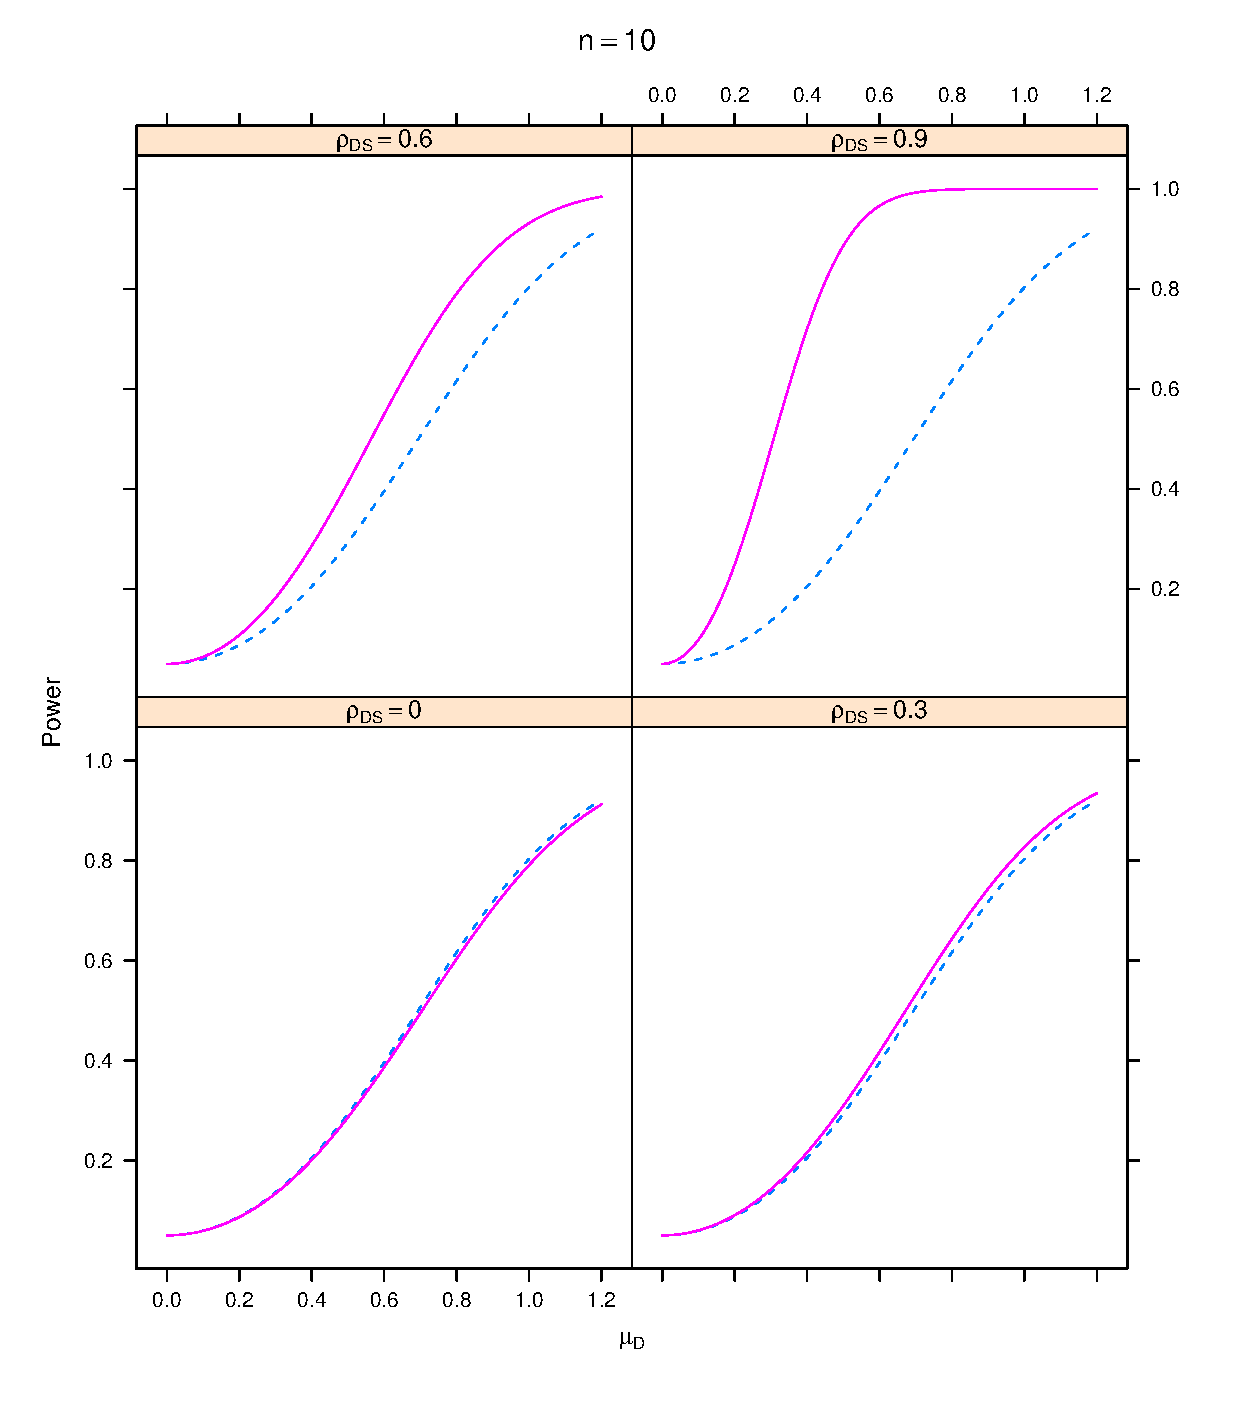
\includegraphics[width=0.47\textwidth]{PowerOne}}
%          \hspace{0.1in}
     \subfigure[][]{
     \label{PowerTwo}
          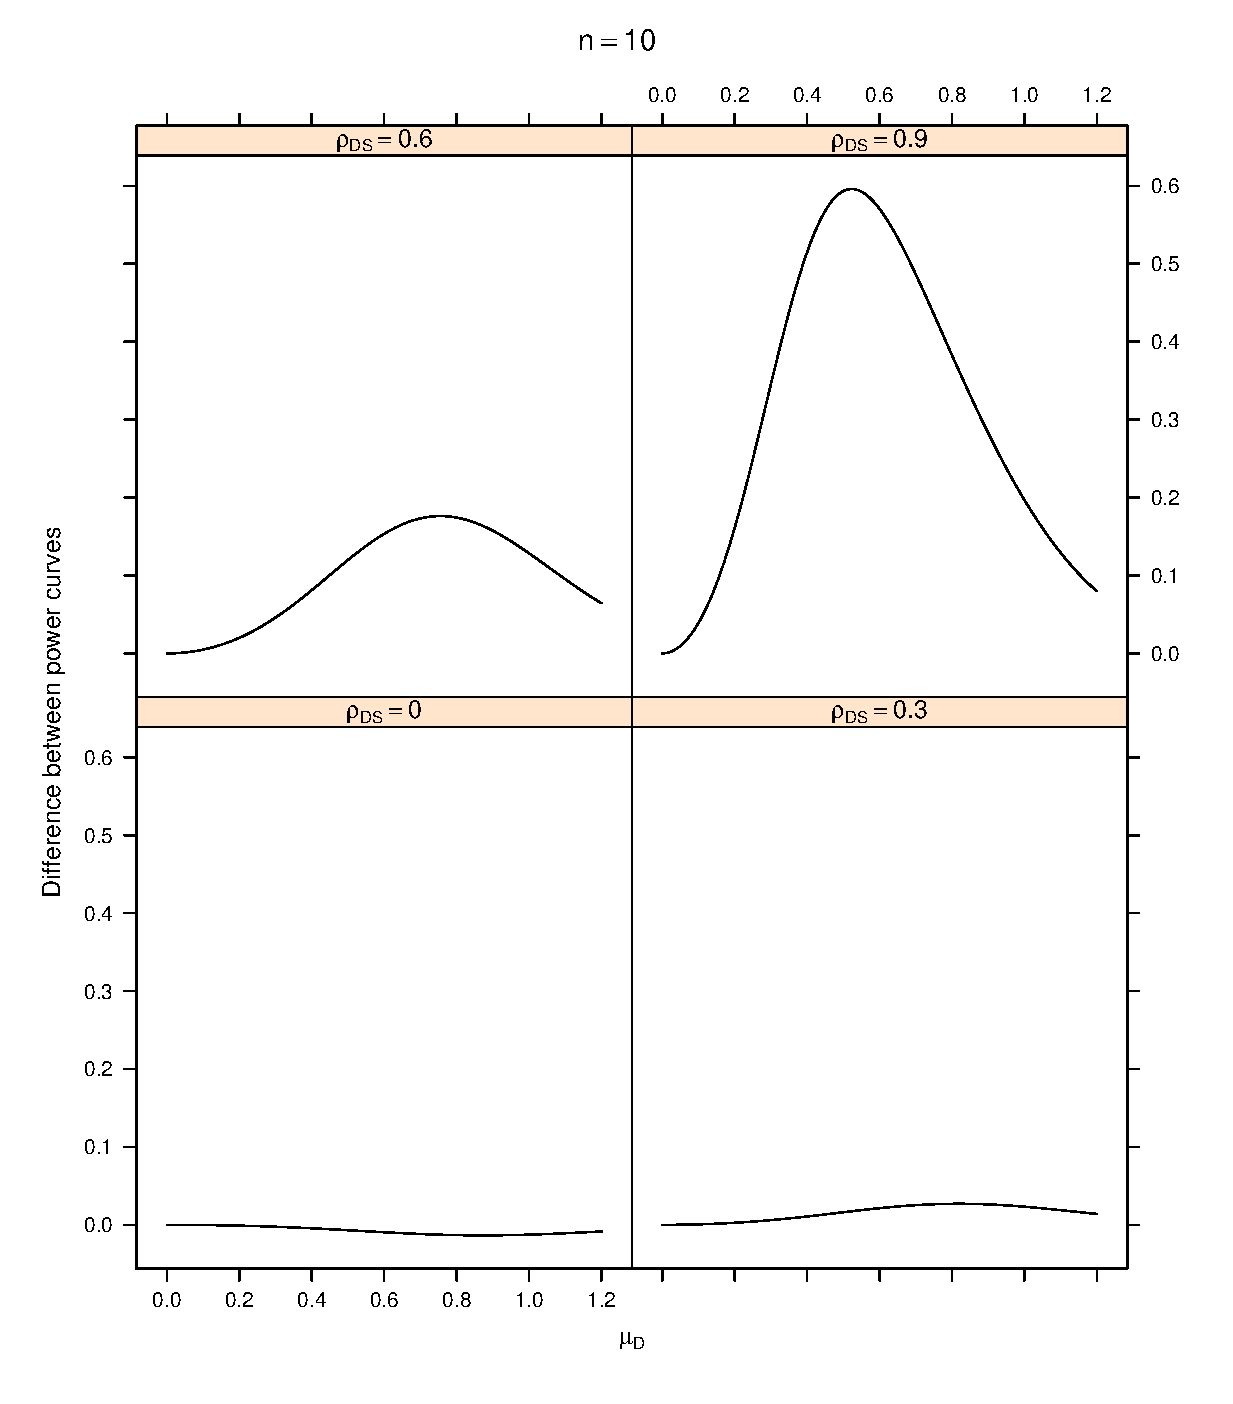
\includegraphics[width=0.47\textwidth]{PowerTwo}}
     \vspace{0.3in}
     \subfigure[][]{
      \label{PowerThree}
          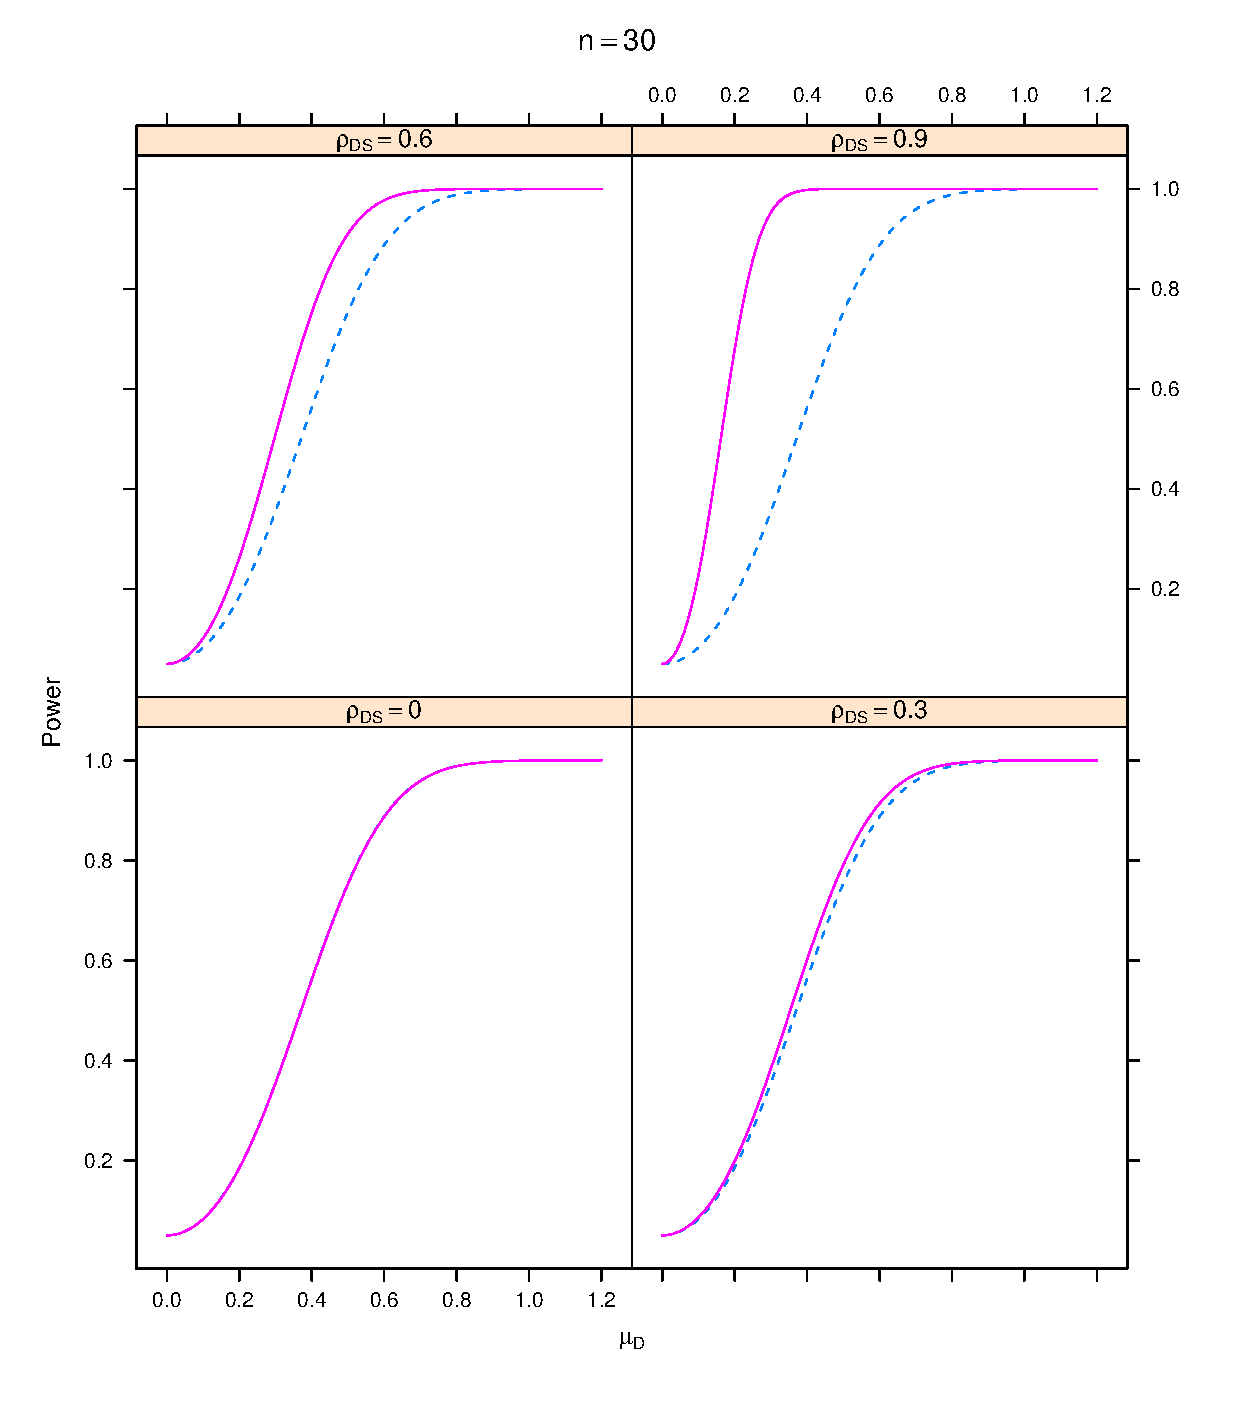
\includegraphics[width=0.47\textwidth]{PowerThree}}
%      \hspace{0.1in}
     \subfigure[][]{
     \label{PowerFour}
          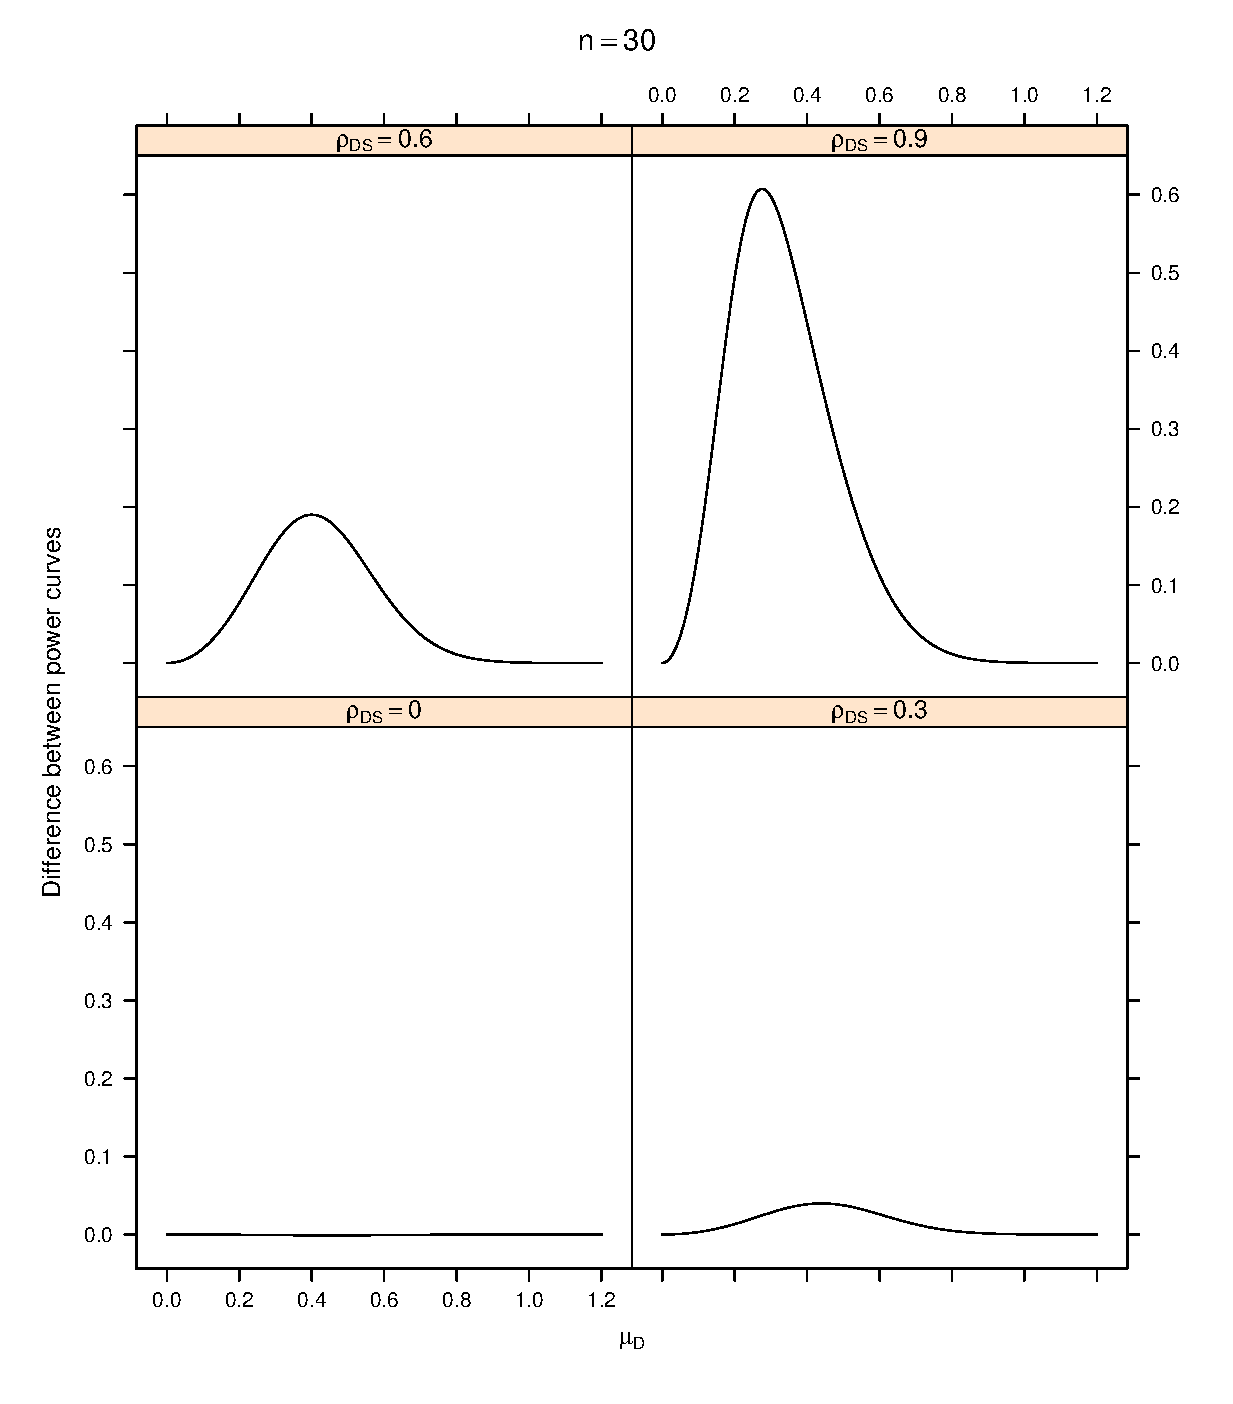
\includegraphics[width=0.47\textwidth]{PowerFour}}
     \caption{The left-hand-side panels \subref{PowerOne} and \subref{PowerThree} show the power functions of the tests of the hypothesis H$'$ using Student's paired-samples \emph{t}-test (dashed line) and the \emph{t}-ratio $t_0^\ast$ (solid line), for sample sizes $n=10$ and $n=30$ respectively. The corresponding differences between these power functions are shown in the right-hand-side panels \subref{PowerTwo} and \subref{PowerFour}. }
\label{PowerCurves}
\end{figure}



\begin{figure}
     \centering
     \makebox{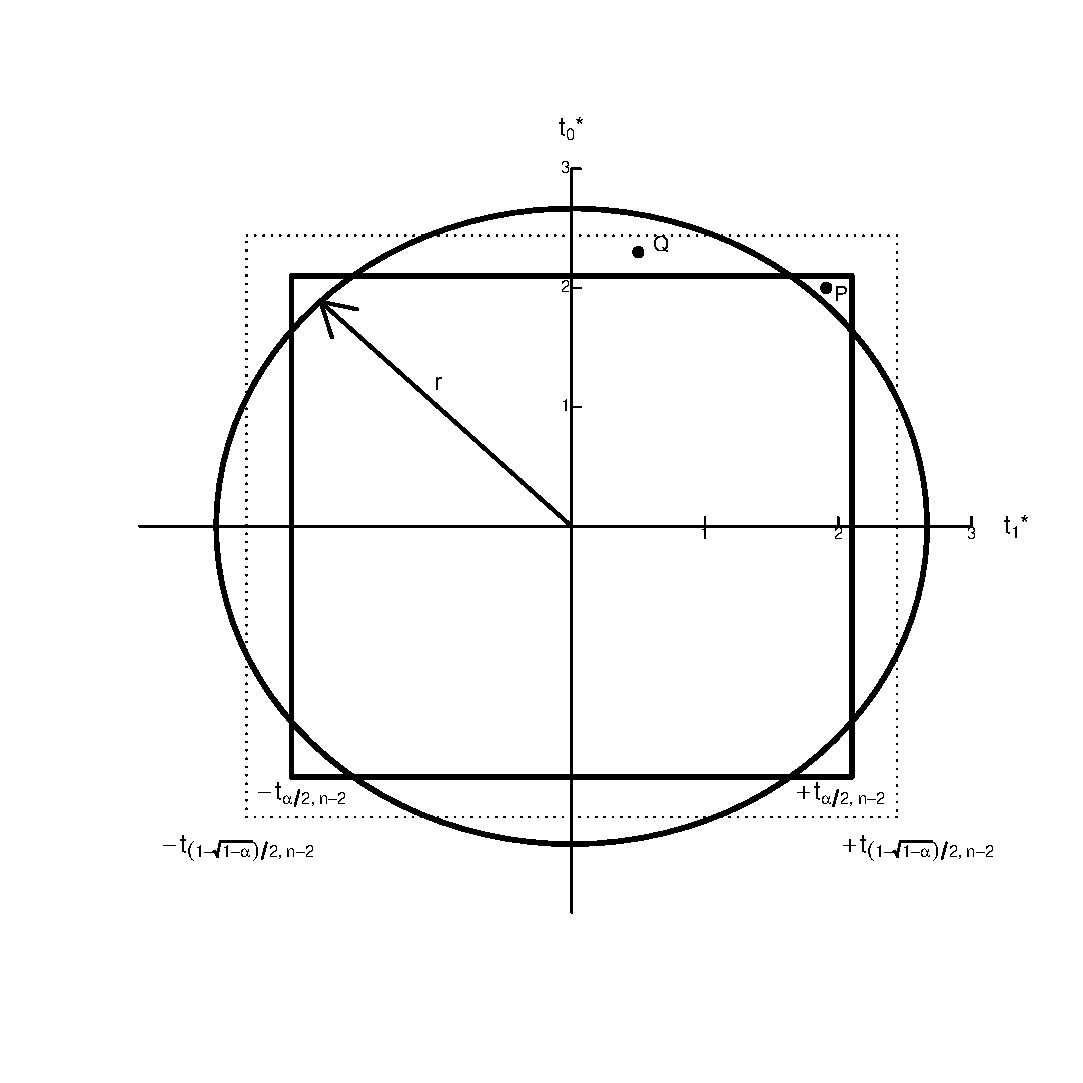
\includegraphics[width=1.0\textwidth]{Regions}}
     \caption{\label{Fig:Rejection:Regions}The circle represents the rejection region
    with type I error probability equal to 5\% for the test of the
    joint hypothesis H: $\beta_0=\beta_1=0$ using the
    Bradley-Blackwood test defined in (\ref{BBHayes}). The inner
    square represents the rejection region with collective type I
    error probability equal to 9.75\% for simultaneous tests on the
    marginal hypotheses H: $\beta_0=0$ and H: $\beta_1=0$ based on
    comparing the \textit{t}-ratios $|t_0^\ast|$ and $|t_1^\ast|$ to
    the cutoff value $t_{\alpha/2,n-2}.$ The outer square represents
    the rejection region with collective type I error probability
    equal to 5\% for simultaneous tests on the marginal hypotheses H:
    $\beta_0=0$ and H: $\beta_1=0$ based on comparing the
    \textit{t}-ratios $|t_0^\ast|$ and $|t_1^\ast|$ to the cutoff
    value $t_{(1-\sqrt{1-\alpha}\ )/2,n-2}.$}
\end{figure}


\begin{figure}
     \centering
     \subfigure[][]{
     \label{Fig3a}
          \hspace{0.15in} 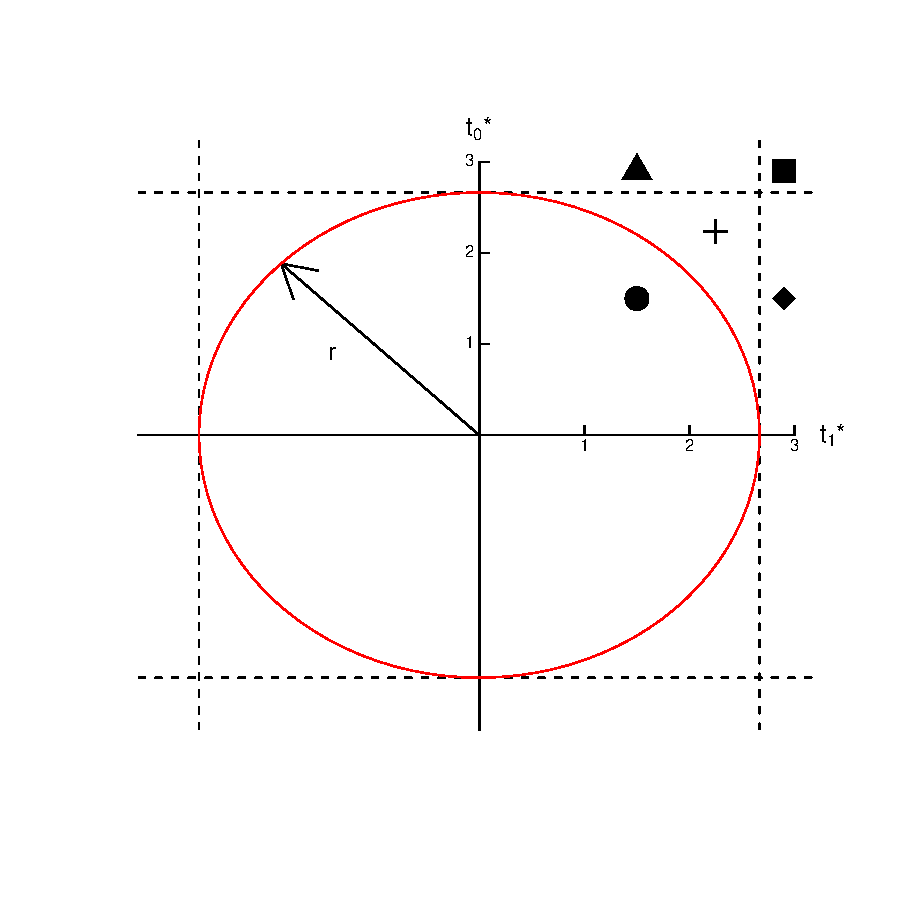
\includegraphics[height=0.36\textwidth]{Fig3a}}
     \subfigure[][]{
      \label{Fig3b}
          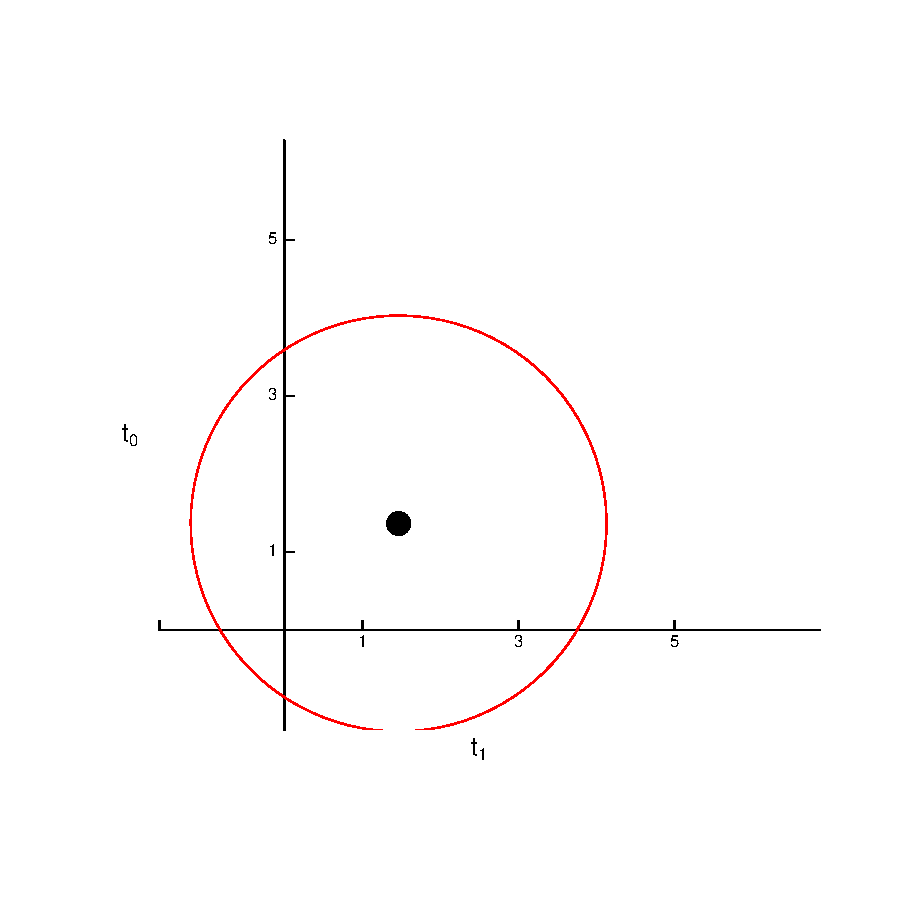
\includegraphics[height=0.42\textwidth]{Fig3b}}
     \subfigure[][]{
     \label{Fig3c}
          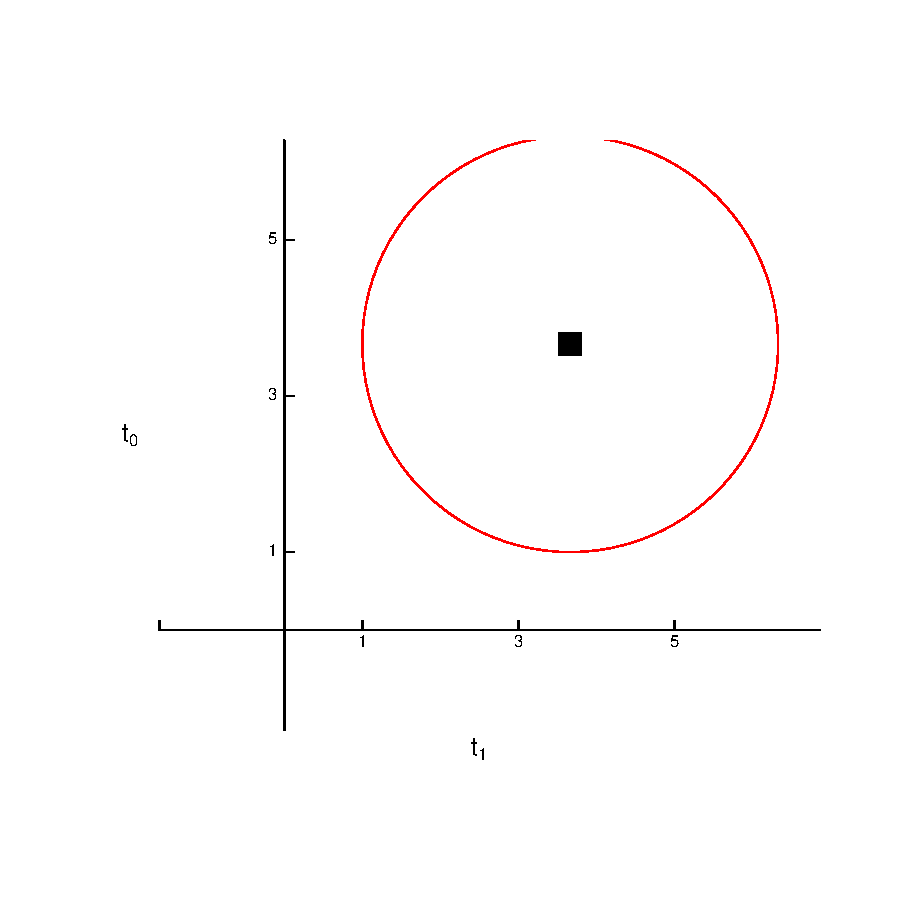
\includegraphics[height=0.42\textwidth]{Fig3c}}
     \subfigure[][]{
      \label{Fig3d}
          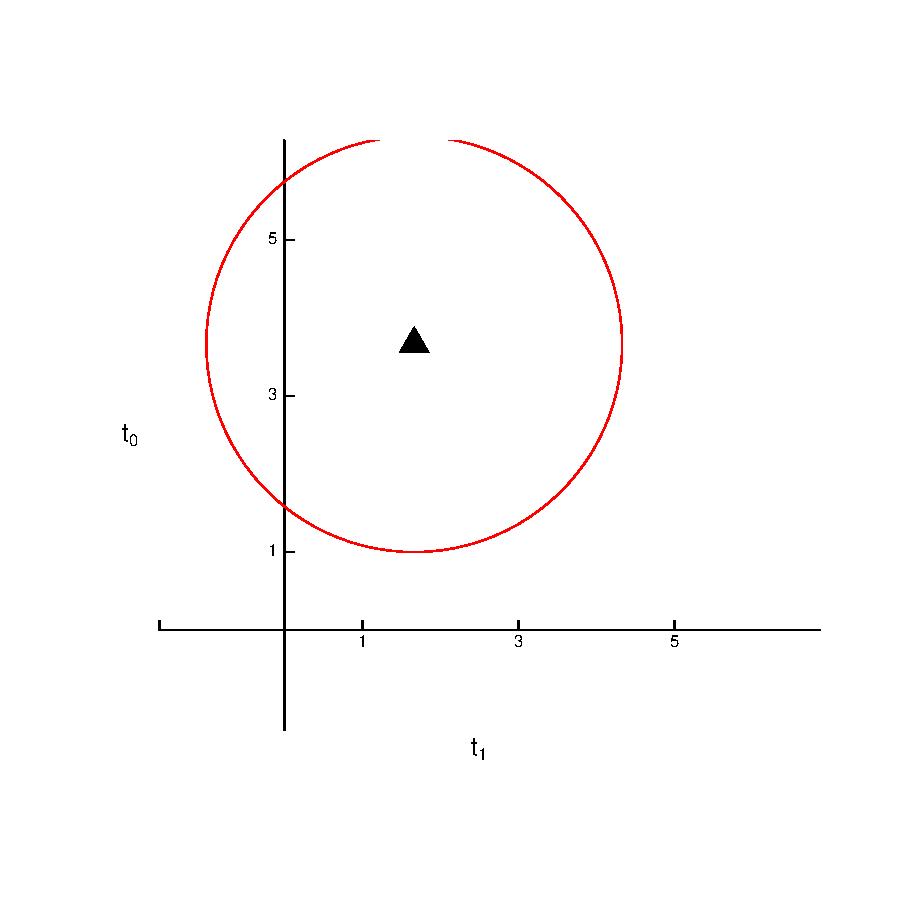
\includegraphics[height=0.42\textwidth]{Fig3d}}
    \subfigure[][]{
     \label{Fig3e}
          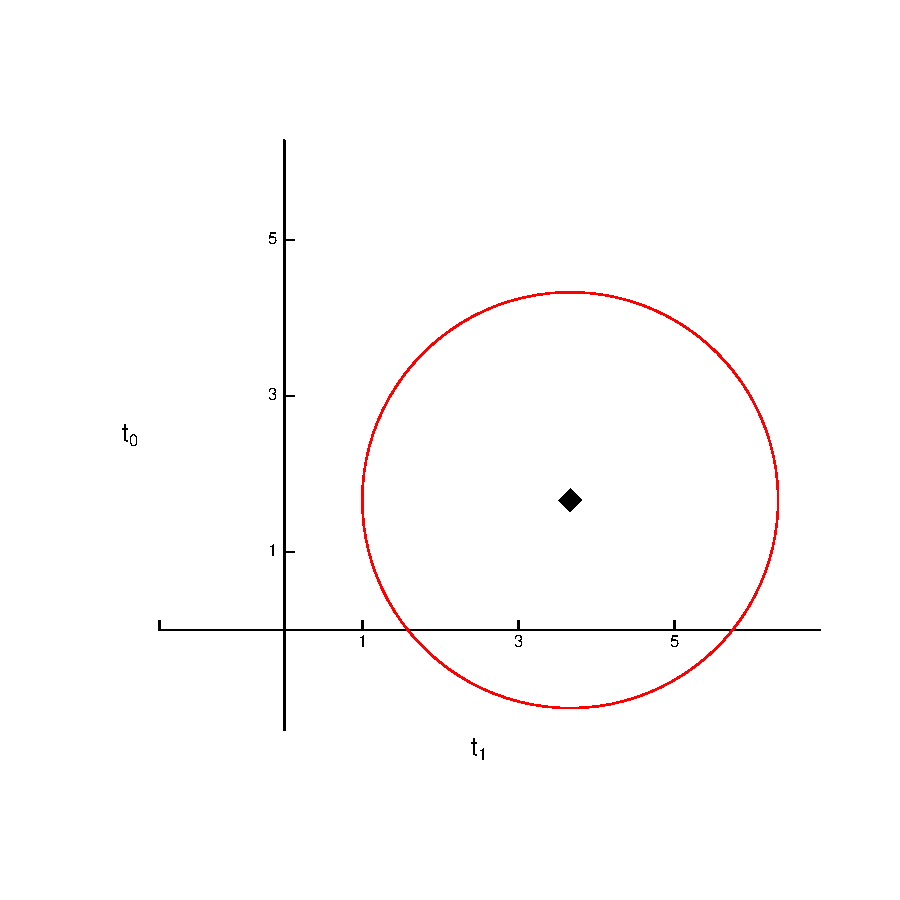
\includegraphics[height=0.42\textwidth]{Fig3e}}
     \subfigure[][]{
      \label{Fig3f}
          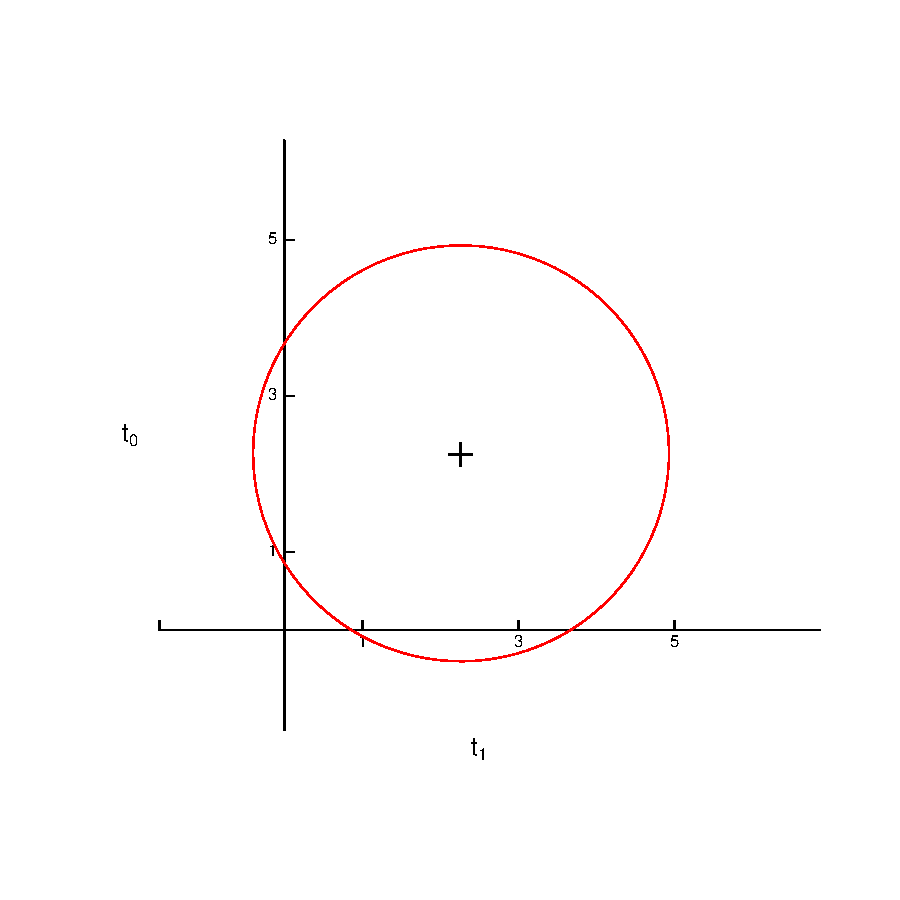
\includegraphics[height=0.42\textwidth]{Fig3f}}
     \caption{Left Joint confidence regions on the test
statistics $(t_0,t_1).$.} \label{FIG3}
\end{figure}


\end{document}
